% Setup -------------------------------

\documentclass[a4paper]{report}
\usepackage[a4paper, total={6in, 10in}]{geometry}
\setcounter{secnumdepth}{3}
\setcounter{tocdepth}{3}

\PassOptionsToPackage{hyphens}{url}
\usepackage{hyperref}

% Images package
\usepackage{graphicx}

% R language style
\usepackage[svgnames]{xcolor}
\usepackage{listings}

\lstset{language=R,
    basicstyle=\small\ttfamily,
    stringstyle=\color{DarkGreen},
    otherkeywords={0,1,2,3,4,5,6,7,8,9},
    morekeywords={TRUE,FALSE},
    deletekeywords={data,frame,length,as,character},
    keywordstyle=\color{blue},
    commentstyle=\color{DarkGreen},
}

% Encoding
%--------------------------------------
\usepackage[T1]{fontenc}
\usepackage[utf8]{inputenc}
%--------------------------------------

% Portuguese-specific commands
%--------------------------------------
\usepackage[portuguese]{babel}
%--------------------------------------

% Hyphenation rules
%--------------------------------------
\usepackage{hyphenat}
%--------------------------------------

% Capa do relatório

\title{
	Aprendizagem Automática I
	\\ \Large{\textbf{Projeto de Avaliação}}
	\\ -
	\\ Mestrado em Engenharia Informática
	\\ \large{Universidade do Minho}
	\\ Relatório
}
\author{
	\begin{tabular}{ll}
		\textbf{Grupo}
		\\\hline
		PG41081 & José Alberto Martins Boticas
		\\
		PG41091 & Nelson José Dias Teixeira
	\end{tabular}
}

\date{\today}

\begin{document}

\begin{titlepage}
    \maketitle
\end{titlepage}

% Resumo

\begin{abstract}
	Este projeto de avaliação relativo à unidade curricular de Aprendizagem Automática I consiste, globalmente, na aplicação de uma das técnicas abordadas durante as aulas sobre um 
	conjunto de dados. O conjunto de dados mencionado previamente é escolhido sem qualquer tipo de restrição por parte dos elementos do grupo por forma a despoletar o interesse dos 
	mesmos durante a análise estatística dos dados presentes. Como tal, durante a execução deste trabalho prático (cuja unidade curricular integra o perfil de Ciência de Dados), 
	surge uma motivação extra na interpretação dos resultados obtidos.
\end{abstract}

% Índice

\tableofcontents

% Introdução

\chapter{Introdução} \label{intro}
\large{
    \section{Apresentação da base de dados escolhida}
	A base de dados escolhida pelos dois elementos que constituem este grupo diz respeito a registos clínicos ou hospitalares de \textit{Cleveland} com informação relativa à presença ou 
	ausência de doenças cardíacas. Nesta pode-se encontrar exatamente 14 atributos, como por exemplo a idade e o sexo de uma dada pessoa bem como registos da sua pressão arterial. 
	
	\section{Contextualização}
	Apesar dos progressos consideráveis na luta contra as doenças cardiovasculares, estas continuam a ser a principal causa de morte na Europa. A alimentação inadequada é responsável por 
	cerca de metade das mortes e da incapacidade causada pelas doenças cardiovasculares.
	
	Em Portugal, cerca de 35 mil portugueses morrem anualmente por doenças cardiovasculares, que continuam a ser a principal causa de morte e representam um terço de toda a mortalidade da 
	população, embora muitas dessas mortes e desse sofrimento prolongado pudessem ser evitados por uma mudança simples nos hábitos alimentares.
	
	Com estes dados, os elementos que compõem este grupo ficaram sensibilizados acerca deste tema e mostraram-se interessados em investigar os fatores que de facto influenciam o aparecimento 
	de doenças cardíacas.

	\section{Definição das variáveis}
	No que diz respeito às variáveis associadas a esta base de dados foi relativamente acessível executar a sua análise. Contudo, o significado dos nomes atribuídos a cada uma das mesmas 
	não é de todo trivial. Desta forma, exibe-se de seguida de forma mais detalhada o que cada uma das variáveis representa:
    \begin{itemize}
	    \item \textbf{age}: idade de uma determinada pessoa em anos;
		\item \textbf{sex}: sexo de uma determinada pessoa:
		\begin{itemize}
			\item 1 : masculino;
			\item 0 : feminino.
		\end{itemize}
	    \item \textbf{cp}: tipo de dor no peito (4 tipos):
	    \begin{itemize}
			\item 1 : angina típica;
			\item 2 : angina atípica;
			\item 3 : dor não anginal;
			\item 4 : assintomática.
		\end{itemize}
	    \item \textbf{trestbps}: pressão arterial em repouso (em \textit{mm} \textit{Hg} de uma determinada pessoa na admissão no hospital);
	    \item \textbf{chol}: medição do colesterol de uma determinada pessoa em \textit{mg/dl};
		\item \textbf{fbs}: açúcar no sangue em jejum > 120 \textit{mg/dl} da pessoa em causa:
		\begin{itemize}
			\item 1 : verdadeiro;
			\item 0 : falso.
		\end{itemize}
	    \item \textbf{restecg}: resultados eletrocardiográficos em repouso de uma pessoa:
	    \begin{itemize}
			\item 0 : normal;
			\item 1 : com anormalidade da onda \textit{ST-T};
			\item 2 : com provável ou definida hipertrofia ventricular esquerda pelo critério de Estes.
		\end{itemize}
	    \item \textbf{thalach}: frequência cardíaca máxima alcançada;
		\item \textbf{exang}: angina induzida pelo exercício:
		\begin{itemize}
			\item 1 : sim;
			\item 0 : não.
		\end{itemize}
	    \item \textbf{oldpeak}: depressão \textit{ST} induzida por exercício em relação ao repouso;
	    \item \textbf{slope}: a inclinação do segmento ST do pico do exercício:
	    \begin{itemize}
			\item 1 : ascendente;
			\item 2 : plano (constante);
			\item 3 : descendente.
		\end{itemize}
	    \item \textbf{ca}: número de vasos principais (0-3);
		\item \textbf{thal}: distúrbio sanguíneo denominado por talassemia:
		\begin{itemize}
			\item 3 : normal;
			\item 6 : defeito fixo;
			\item 7 : defeito reversível.
		\end{itemize}
	    \item \textbf{target}: doença cardíaca (ver distribuição na figura \ref{fig:barplot}):
	    \begin{itemize}
			\item 1 : sim;
			\item 0 : não.
		\end{itemize}

		\begin{figure}[h!]
			\centering
			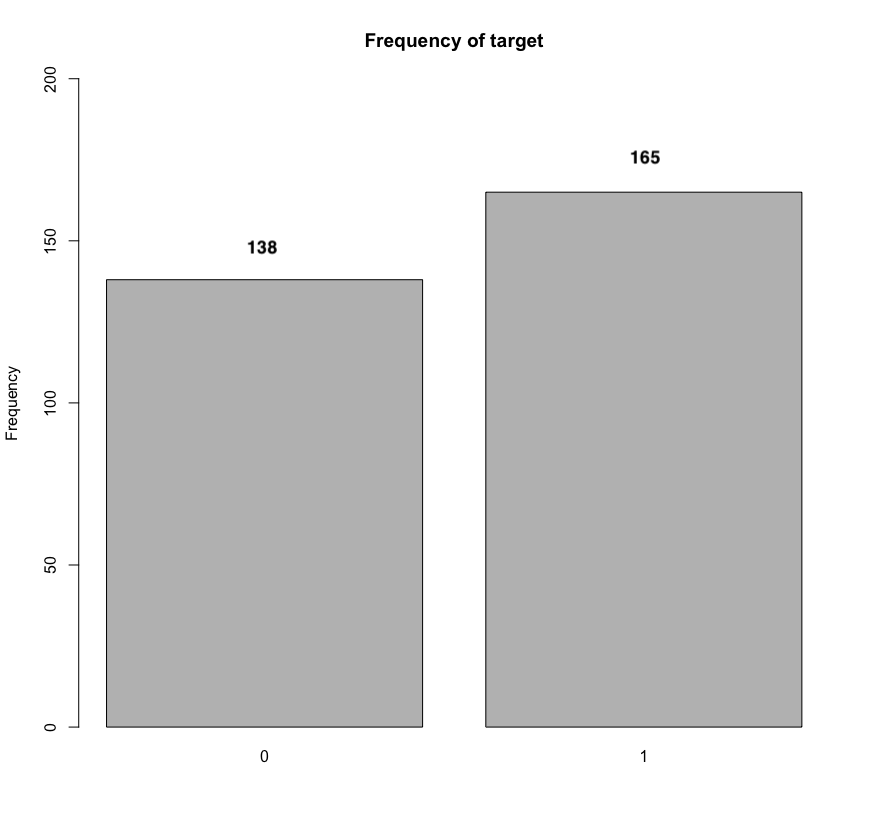
\includegraphics[scale=0.4]{images/barplot.png}
			\caption{\textit{Barplot} da variável \textit{target}}
			\label{fig:barplot}
		\end{figure}

    \end{itemize}
	
	Ainda relativamente às incógnitas presentes na base de dados foi possível identificar tanto as variáveis quantitativas como as variáveis qualitativas ou categóricas. 
	Apresenta-se de seguida o tipo de cada uma das variáveis presentes:
	\begin{center}
		\begin{tabular}{ | l | l | }
		\hline
		\textbf{Nome da variável} & \textbf{Tipo de variável} \\ \hline
		age & Quantitativa discreta \\ \hline
		sex & Qualitativa ordinal \\ \hline
		cp & Qualitativa ordinal \\ \hline
		trestbps & Quantitativa discreta \\ \hline
		chol & Quantitativa discreta \\ \hline
		fbs & Qualitativa ordinal \\ \hline
		restecg & Qualitativa ordinal \\ \hline
		thalach & Quantitativa discreta \\ \hline
		exang & Qualitativa ordinal \\ \hline
		oldpeak & Quantitativa contínua \\ \hline
		slope & Qualitativa ordinal \\ \hline
		ca & Quantitativa discreta \\ \hline
		thal & Qualitativa ordinal \\ \hline
		target & Qualitativa ordinal \\ \hline
		\end{tabular}
	\end{center}
	
	\section{Objetivo de análise}
	Perante esta base de dados, os elementos que integram este grupo procuram, com a informação disponível, prever se uma determinada pessoa possui ou não uma doença cardíaca. Consequentemente,
	a variável de interesse para realizar este estudo corresponde à incógnita \textit{target}, pelo que o problema em causa é de classificação.
	Para além deste objetivo, vamos também perceber se existem outros fatores relativos ao coração que permitem prever certos eventos cardiovasculares. 
	
	Após traçarmos o objetivo principal na análise sobre a base de dados em causa, surgiram algumas questões da nossa parte. Apresentam-se de seguida as mesmas:
	\begin{enumerate}
	    \item O que influencia o aparecimento de uma doença cardíaca?
	    \item Que fatores indicam a presença de uma doença cardíaca?
		\item Podemos prever a existência de uma doença cardíaca com os indicadores expostos?
	\end{enumerate}
	
	Consequentemente, por forma a responder a estas questões, é necessário especificar um modelo estatístico que se adequa a este contexto. Como tal, na próxima secção deste documento, 
	é apresentado o modelo requerido.
}

\chapter{Metodologia}
\large{
	Tal como o nome deste capítulo indica, nesta secção do documento será feita a exposição do modelo adotado pelo grupo para a análise correta dos dados presentes. À semelhança do que foi dito 
	anteriormente, a variável de interesse presente neste conjunto de dados corresponde à incógnita \textit{\textbf{target}}. Uma vez que a mesma é uma variável qualitativa ordinal, temos que o 
	problema em causa é um problema de \textbf{classificação}. Como tal, a técnica de regressão adotada para modelar esta base de dados é nada mais nada menos do que a \textbf{regressão logística}.

	\section{Escolha do melhor modelo}
	\subsection{Filosofia}

	Foram testados diversos modelos de regressão logística para se descobrir qual deles seria o melhor.
	
	O primeiro deles foi, desde logo, o mais óbvio, com todas as variáveis da base de dados como preditores:

	\begin{verbatim}
	    model.1 <- glm(target ~ ., family = binomial, data = database)
	\end{verbatim}

	A partir daqui, criaram-se diversos modelos. Uma a uma, retiram-se as variáveis não estatisticamente significativas.
	Depois de retiradas 5 variáveis, todas as variáveis apresentavam significância, embora uma delas apenas a 10\%.
	Por isso, tomou-se a decisão de se experimentar mais um modelo, retirando a dita variável.
	
	Por fim, tentou-se ainda um outro modelo, retirando do modelo inicial todas as variáveis que se revelaram não estatisticamente significativas no mesmo.
	Repetiu-se o processo anterior, sendo que foi apenas gerado um modelo, mas o mesmo foi descartado por ser idêntico a outro já gerado.

	Embora já com sete modelos, foi decidida a tentativa de uma nova abordagem. 
	Assim, testaram-se modelos variável a variável. A partir destes, escolheram-se as variáveis que tivessem significância a 0.1\% (máxima medida do \textit{R}).
	Com estas, gerou-se um novo modelo. De realçar que o mesmo é diferente de todos os testados anteriormente.

	A remoção de variáveis não estatisticamente significativas gerou um novo modelo, mas o mesmo foi descartado por ser igual a um alcançado anteriormente.


	\subsection{Modelos}

	\begin{center}
		\begin{tabular}{ || l || c | c | c | c | c | c | c | c || }
		\hline
		\textbf{Modelo} & \textbf{1} & \textbf{2} & \textbf{3} & \textbf{4} & \textbf{5} & \textbf{6} & \textbf{7} & \textbf{8} \\
		\hline
		\hline
		\textbf{age} 		& x & x &   &	&	&	&	& x	\\
		\hline
		\textbf{sex} 		& x & x & x & x	& x	& x	& x	& x	\\
		\hline
		\textbf{cp} 		& x & x & x	& x	& x	& x	& x	& x	\\
		\hline
		\textbf{trestbps} 	& x & x & x & x	& x	& x	& x	& x	\\
		\hline
		\textbf{chol} 		& x & x & x &	&	&	&	& 	\\
		\hline
		\textbf{fbs} 		& x &   &   &	&	&	&	& 	\\
		\hline
		\textbf{restecg} 	& x & x & x & x	& x	&	& 	&	\\
		\hline
		\textbf{thalach} 	& x & x & x & x	& x	& x	& x	& x	\\
		\hline
		\textbf{exang} 		& x & x & x & x & x	& x	& x	& x	\\
		\hline
		\textbf{oldpeak} 	& x & x & x & x & x	& x	& x	& x	\\
		\hline
		\textbf{slope} 		& x & x & x & x	&	&	& x	& x	\\
		\hline
		\textbf{ca} 		& x & x & x & x	& x	& x & x	& x	\\
		\hline
		\textbf{thal} 		& x & x & x & x	& x	& x	& x	& x	\\
		\hline
		\end{tabular}
	\end{center}

	Nesta tabela pode-se constatar todos os modelos considerados pelos elementos deste grupo para ajustar o conjunto de dados em causa e, ainda, os preditores incluídos nos mesmos.


	\subsection{Tomada de decisão}

	Desenvolvidos os modelos, procedeu-se ao seu estudo. Foram feitas, entre outras, duas análises principais:
	\begin{itemize}
		\item a percentagem de predições corretas, com recurso à função \begin{verbatim} predict(., type="response") \end{verbatim} e usando como ponto de corte de probabilidade de doença 55\%;
		\item o erro médio dado pela avaliação \textit{cross-validation - leave-one-out}, sendo esse erro médio a proporção de classificações corretas, usando o mesmo ponto de corte (55\%).
	\end{itemize}
	\begin{center}
		\begin{tabular}{ | c | c | c | }
		\hline
		\textbf{Modelo} & \textbf{Predições corretas} & \textbf{Erro médio - Leave-one-out} \\ 
		\hline
		\textbf{1} & 85.48\% & 15.18\% \\ 
		\hline
		\textbf{2} & 85.48\% & 14.85\% \\
		\hline
		\textbf{3} & 85.48\% & 14.52\% \\
		\hline
		\textbf{4} & 85.81\% & 13.86\% \\
		\hline
		\textbf{5} & 85.81\% & 14.52\% \\
		\hline
		\textbf{6} & 84.49\% & 15.51\% \\
		\hline
		\textbf{7} & 85.81\% & 14.85\% \\
		\hline								   	
		\textbf{8} & 86.14\% & 14.19\% \\
		\hline
		\end{tabular}
	\end{center}

	Destas análises, é possível perceber que os modelos têm resultados semelhantes. No entanto, é possível perceber que alguns deles se destacam.

	Vamos então destacar dois destes modelos: \textbf{4} e \textbf{8}. O primeiro destaca-se pela proporção de erro médio, com a técnica de \textit{leave-one-out}, mais baixa.
	O último destaca-se pela proporção de classificações corretas, utilizando toda a base de dados, mais elevada.

	Comparando estes modelos, percebemos que a decisão por um deles se prenderá pela importância que dermos a cada uma das análises.
	Na opinião dos autores deste relatório, a segunda (erro médio) acaba por ser a mais relevante, uma vez que se avalia a capacidade do modelo prever dados que não pertencem à base de dados que serviu de treino.

	Portanto, o modelo escolhido é o modelo número 4.
}

\chapter{Resultados}
\large{
	Respondamos às perguntas feitas no início deste relatório:
	\begin{enumerate}
		\item \textbf{O que influencia o aparecimento de uma doença cardíaca?} \\
		Ao contrário do que se poderia pensar, os níveis de colesterol não parecem ser um bom indicador da presença de uma doença cardíaca, embora seja possível, 
		através do estudo do primeiro modelo, perceber que níveis de colesterol superiores a 120\textit{mg/dl} aumentam a probabilidade.
		Por outro lado, a pressão arterial e a existência de doenças de sangue, do grupo talassemia, parecem ser fatores que influenciam o aparecimento destas doenças, 
		pelo que um cuidado acompanhamento destes fatores pode ser importante para evitar uma doença cardíaca ou o diagnóstico precoce de uma. \\

		A idade poderá ser um fator a ter em conta no aparecimento de uma doença cardíaca. No entanto, neste caso, não foi relevante na especificação dos modelos.
		Isto pode ser explicado pelo facto de a base de dados não ter uma boa representação neste campo, uma vez que as amostras estão compreendidas num curto intervalo, tal 
		como se pode ver na figura \ref{fig:histogram}.

		\begin{figure}[h!]
			\centering
			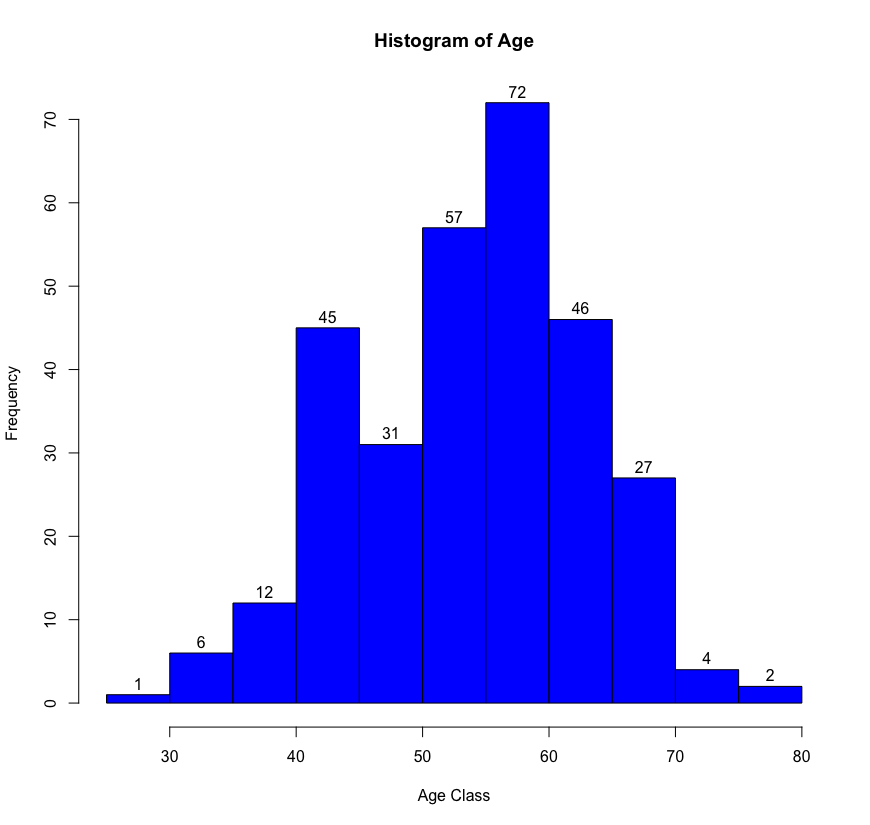
\includegraphics[scale=0.4]{images/histogram.png}
			\caption{Histograma da variável \textit{age}}
			\label{fig:histogram}
		\end{figure}

		\item \textbf{Que fatores podem indicar a presença de doença cardíaca?} \\
		Através do estudo realizado, é possível perceber que a resposta ao exercício físico pode ser um indicador que permita identificar uma doença cardíaca.
		Mais concretamente, deve ter-se em atenção a angina (dor torácica) induzida pelo exercício físico, a frequência cardíaca máxima alcançada e a inclinação do segmento ST no eletrocardiograma, no pico do exercício.
		Obviamente que, tal como referido anteriormente, a presença de uma doença sanguínea também dar pistas importantes nesse sentido.
		Por fim, o número de vasos sanguíneos também aparenta ser um bom indicador da presença de uma doença cardíaca. \\

		\item \textbf{Podemos prever a existência de uma doença cardíaca com os indicadores expostos?} \\
		O estudo indica que poderá ser possível prever a existência de uma doença cardíaca, mas indica que a fiabilidade não é tão elevada como se gostaria.
		No entanto, vários fatores podem influenciar os valores conseguidos, como o tamanho da base de dados, que parece ser algo curta (303 entradas).
		Com o mesmo tipo de preditores e uma base de dados mais extensa, é de prever melhorias nas avaliações.

		Mas será isto necessário? Não conseguirá um médico especializado, com recurso aos mesmos dados, identificar uma doença cardíaca num paciente?
	\end{enumerate}
}

\chapter{Conclusão}
\large{
	Após a apresentação da metodologia e dos resultados obtidos durante análise estatística desta base de dados, dá-se por concluído a realização deste trabalho prático. 
	Com o modelo implementado (e ainda outros desenvolvidos), foi possível dar resposta às perguntas inicialmente traçadas, extraindo informação relevante para a compreensão e interpretação do contexto em causa. 
	Consequentemente, foi também possível alcançar os objectivos delineados na introdução deste documento. 
	
	De notar também que apesar da dimensão reduzida desta base de dados foi possível especificar um modelo adequado para o efeito, ainda que o mesmo não seja o melhor. 
	Uma base de dados mais extensa pode ser a resposta para melhores predições.

	Foi ainda possível concluir que nem todas as variáveis da base de dados são relevantes na previsão da existência de uma doença cardíaca, pelo que a sua substituição pode ser um passo importante na melhoria dos modelos gerados.
}

\chapter{Webgrafia}
	\begin{itemize}
		\item \textit{Website} indicado pela docente:
		\par \textit{\url{https://www.kaggle.com/datasets}}
        \item \textit{Website} com o resumo da base de dados escolhida:
		\par \textit{\url{https://www.kaggle.com/ronitf/heart-disease-uci}}
		\item \textit{Website} com a informação oficial da base de dados escolhida:
		\par \textit{\url{https://archive.ics.uci.edu/ml/datasets/Heart+Disease}}
	\end{itemize}


\appendix
\chapter{Código dos modelos desenvolvidos}

\begin{lstlisting}[breaklines,basicstyle=\small]
# Carregar a base de dados
db <- read.csv(file="database/heart.csv", header=T)

ncol(db)
nrow(db)
colnames(db)

# Garantir que nao existem valores em falta.
sum(is.na(db))

# ---------------------- MODELOS ----------------------

# todas as variaveis
model.1 = glm(target ~ ., family = binomial, data = db)
summary(model.1)

# sem fbs
model.2 = glm(target ~ age + sex + cp + trestbps + chol + restecg + thalach + exang + oldpeak + slope + ca + thal, data = db, family = binomial)
summary(model.2)

# sem age
model.3 = glm(target ~ sex + cp + trestbps + chol + restecg + thalach + exang + oldpeak + slope + ca + thal, data = db, family = binomial)
summary(model.3) 

# sem chol
model.4 = glm(target ~ sex + cp + trestbps + restecg + thalach + exang + oldpeak + slope + ca + thal, data = db, family = binomial)
summary(model.4)

# sem slope
model.5 = glm(target ~ sex + cp + trestbps + restecg + thalach + exang + oldpeak + ca + thal, data = db, family = binomial)
summary(model.5) # ja sao todas significativas, mas uma e a 10%

# sem restecg, para ficarem todas a 5%
model.6 = glm(target ~ sex + cp + trestbps + thalach + exang + oldpeak + ca + thal, data = db, family = binomial)
summary(model.6) 

# primeiro modelo tirando todas as vars nao significativas
model.7 = glm(target ~ sex + cp + trestbps + thalach + exang + oldpeak + slope + ca + thal, data = db, family = binomial)
summary(model.7)


# ---------------------- TESTES ----------------------

model.test1 <- glm(target ~ age, data = db, family = binomial)
model.test2 <- glm(target ~ sex, data = db, family = binomial)
model.test3 <- glm(target ~ cp, data = db, family = binomial)
model.test4 <- glm(target ~ trestbps, data = db, family = binomial)
model.test5 <- glm(target ~ chol, data = db, family = binomial)
model.test6 <- glm(target ~ fbs, data = db, family = binomial)
model.test7 <- glm(target ~ restecg, data = db, family = binomial)
model.test8 <- glm(target ~ thalach, data = db, family = binomial)
model.test9 <- glm(target ~ exang, data = db, family = binomial)
model.test10 <- glm(target ~ oldpeak, data = db, family = binomial)
model.test11 <- glm(target ~ slope, data = db, family = binomial)
model.test12 <- glm(target ~ ca, data = db, family = binomial)
model.test13 <- glm(target ~ thal, data = db, family = binomial)

# Modelo construido a partir da analise anterior
model.8 = glm(target ~ sex + age + cp + trestbps + thalach + exang + oldpeak + slope + ca + thal, data = db, family = binomial)
summary(model.8)

# Qual o melhor modelo?
# Proporcao de classificacoes corretas
probs.1 = predict(model.1, type = "response"); pred.1 = rep(0, 303); pred.1[probs.1 > 0.55] = 1 
probs.2 = predict(model.2, type = "response"); pred.2 = rep(0, 303); pred.2[probs.2 > 0.55] = 1 
probs.3 = predict(model.3, type = "response"); pred.3 = rep(0, 303); pred.3[probs.3 > 0.55] = 1 
probs.4 = predict(model.4, type = "response"); pred.4 = rep(0, 303); pred.4[probs.4 > 0.55] = 1 
probs.5 = predict(model.5, type = "response"); pred.5 = rep(0, 303); pred.5[probs.5 > 0.55] = 1 
probs.6 = predict(model.6, type = "response"); pred.6 = rep(0, 303); pred.6[probs.6 > 0.55] = 1 
probs.7 = predict(model.7, type = "response"); pred.7 = rep(0, 303); pred.7[probs.7 > 0.55] = 1
probs.8 = predict(model.8, type = "response"); pred.8 = rep(0, 303); pred.8[probs.8 > 0.55] = 1

mean(pred.1 == db$target)
mean(pred.2 == db$target)
mean(pred.3 == db$target)
mean(pred.4 == db$target)
mean(pred.5 == db$target)
mean(pred.6 == db$target)
mean(pred.7 == db$target)
mean(pred.8 == db$target)

# Cross-validation - Leave-one-out
library(boot)

mycost = function(r, pi = 0) mean(abs(r-pi)) > 0.55

cv.err1 = c(); cv.err2 = c(); cv.err3 = c(); cv.err4 = c()
cv.err5 = c(); cv.err6 = c(); cv.err7 = c(); cv.err8 = c()

s = nrow(db)

cv.err1 <- c(cv.err1, cv.glm(db, model.1, cost = mycost, K=s)$delta[1])
cv.err2 <- c(cv.err2, cv.glm(db, model.2, cost = mycost, K=s)$delta[1])
cv.err3 <- c(cv.err3, cv.glm(db, model.3, cost = mycost, K=s)$delta[1])
cv.err4 <- c(cv.err4, cv.glm(db, model.4, cost = mycost, K=s)$delta[1])
cv.err5 <- c(cv.err5, cv.glm(db, model.5, cost = mycost, K=s)$delta[1])
cv.err6 <- c(cv.err6, cv.glm(db, model.6, cost = mycost, K=s)$delta[1])
cv.err7 <- c(cv.err7, cv.glm(db, model.7, cost = mycost, K=s)$delta[1])
cv.err8 <- c(cv.err8, cv.glm(db, model.8, cost = mycost, K=s)$delta[1])
cv.err9 <- c(cv.err9, cv.glm(db, model.9, cost = mycost, K=s)$delta[1])

cv.err1
cv.err2
cv.err3
cv.err4
cv.err5
cv.err6
cv.err7
cv.err8
\end{lstlisting}

\end{document}